\section{Anhang}
\label{sec:Anhang}
\subsection{Abbildungen zur Bestimmung der Viskosität der Luft}
\begin{figure}[H]
    \centering
    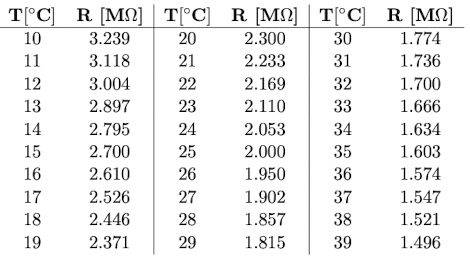
\includegraphics[height=5cm]{content/pics/R_T.png}
    \caption{Tabelle zum Umrechnen des Widerstands des Theromelements in eine Temperatur \cite{v503}.}
    \label{fig:R_T}
\end{figure}
\begin{figure}[H]
    \centering
    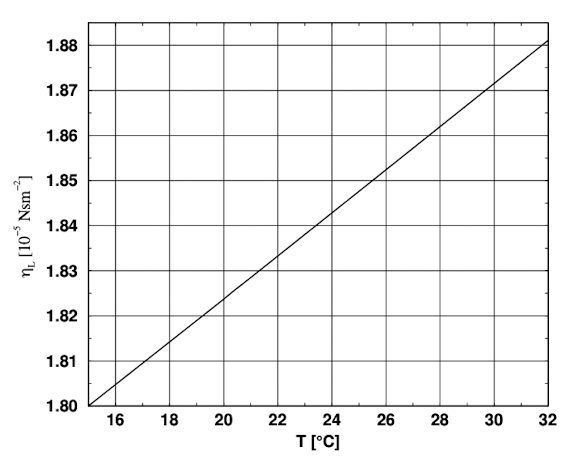
\includegraphics[height=10cm]{content/pics/eta_T.png}
    \caption{Grafik zum Zusammenhang zwischen Temperatur und Viskosität der Luft \cite{v503}.}
    \label{fig:eta_L}
\end{figure}

\subsection{Originaldaten}
\centering
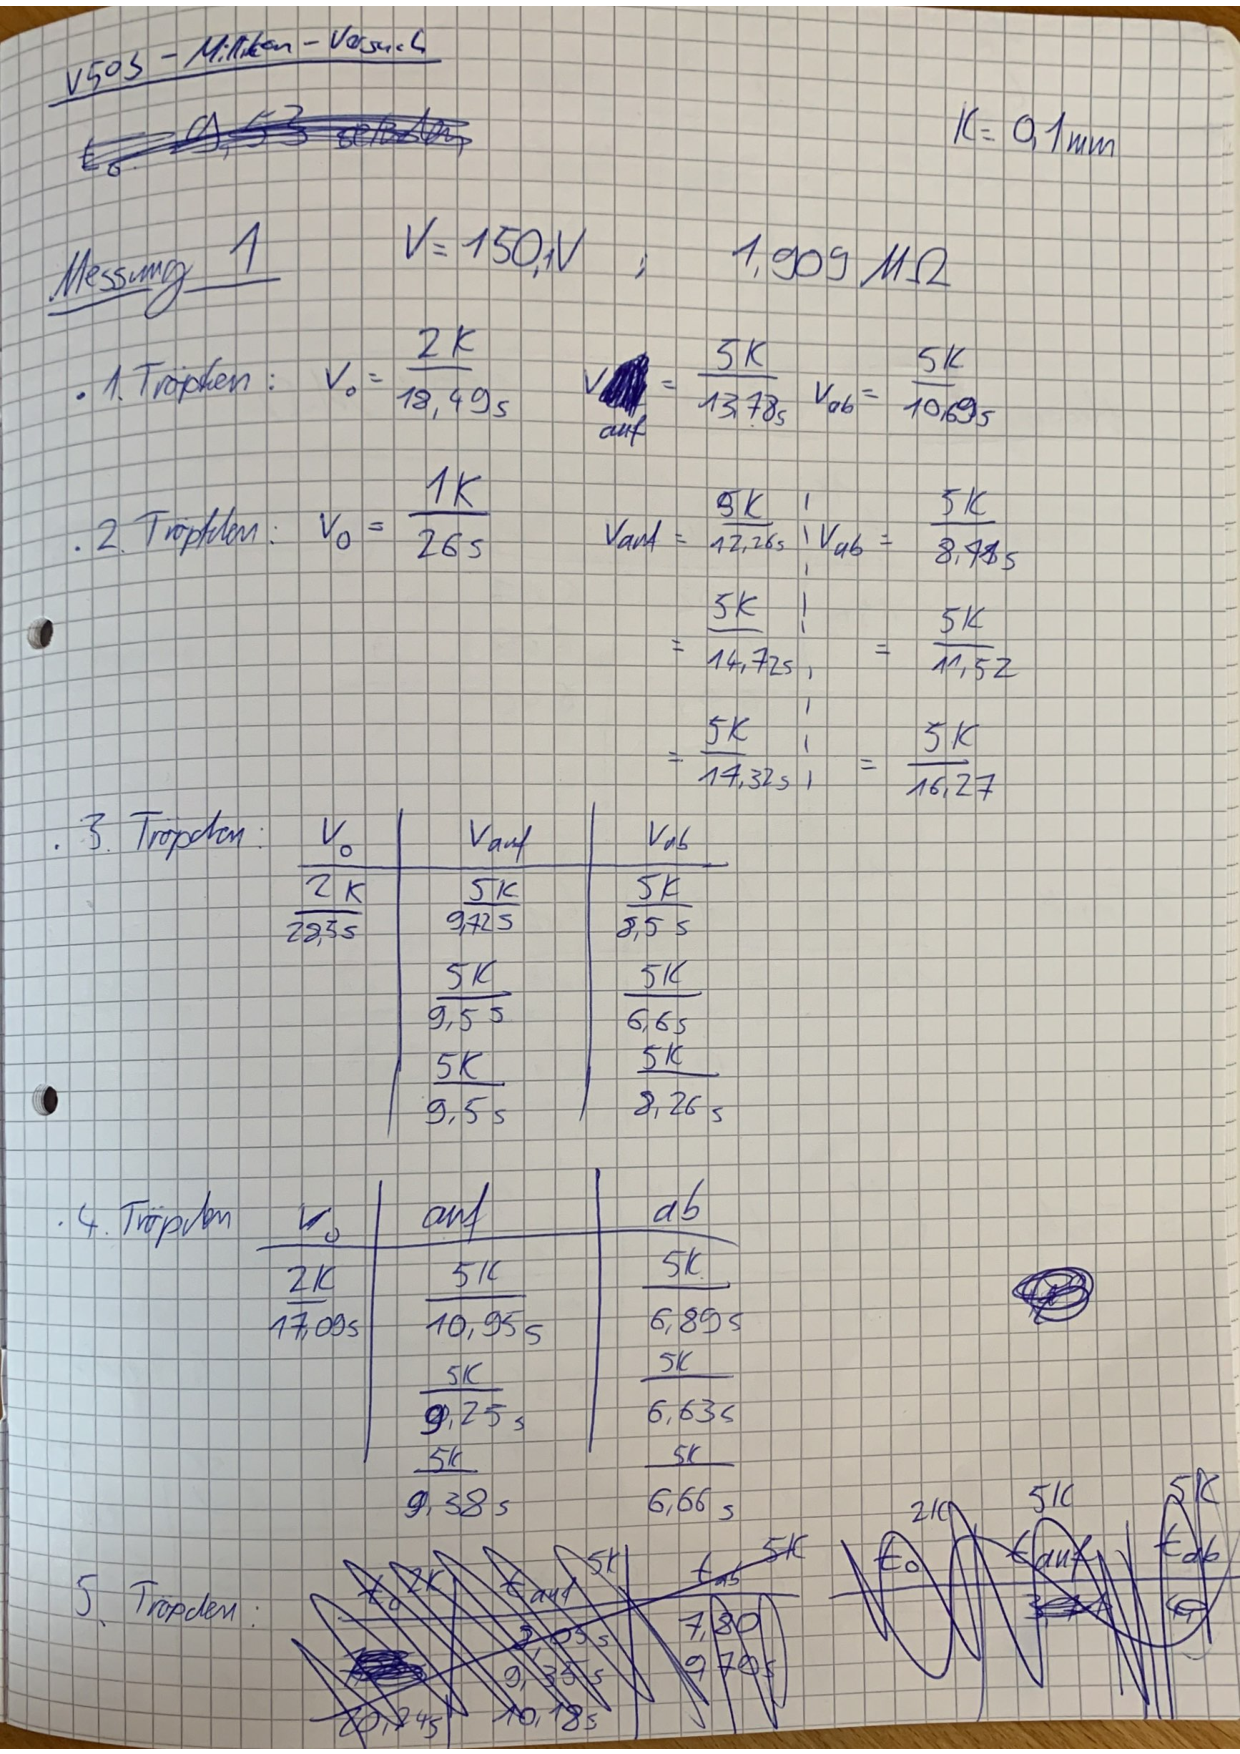
\includegraphics[height=18cm]{content/pics/originaldaten/Originaldaten_1.pdf}
\newpage
\centering
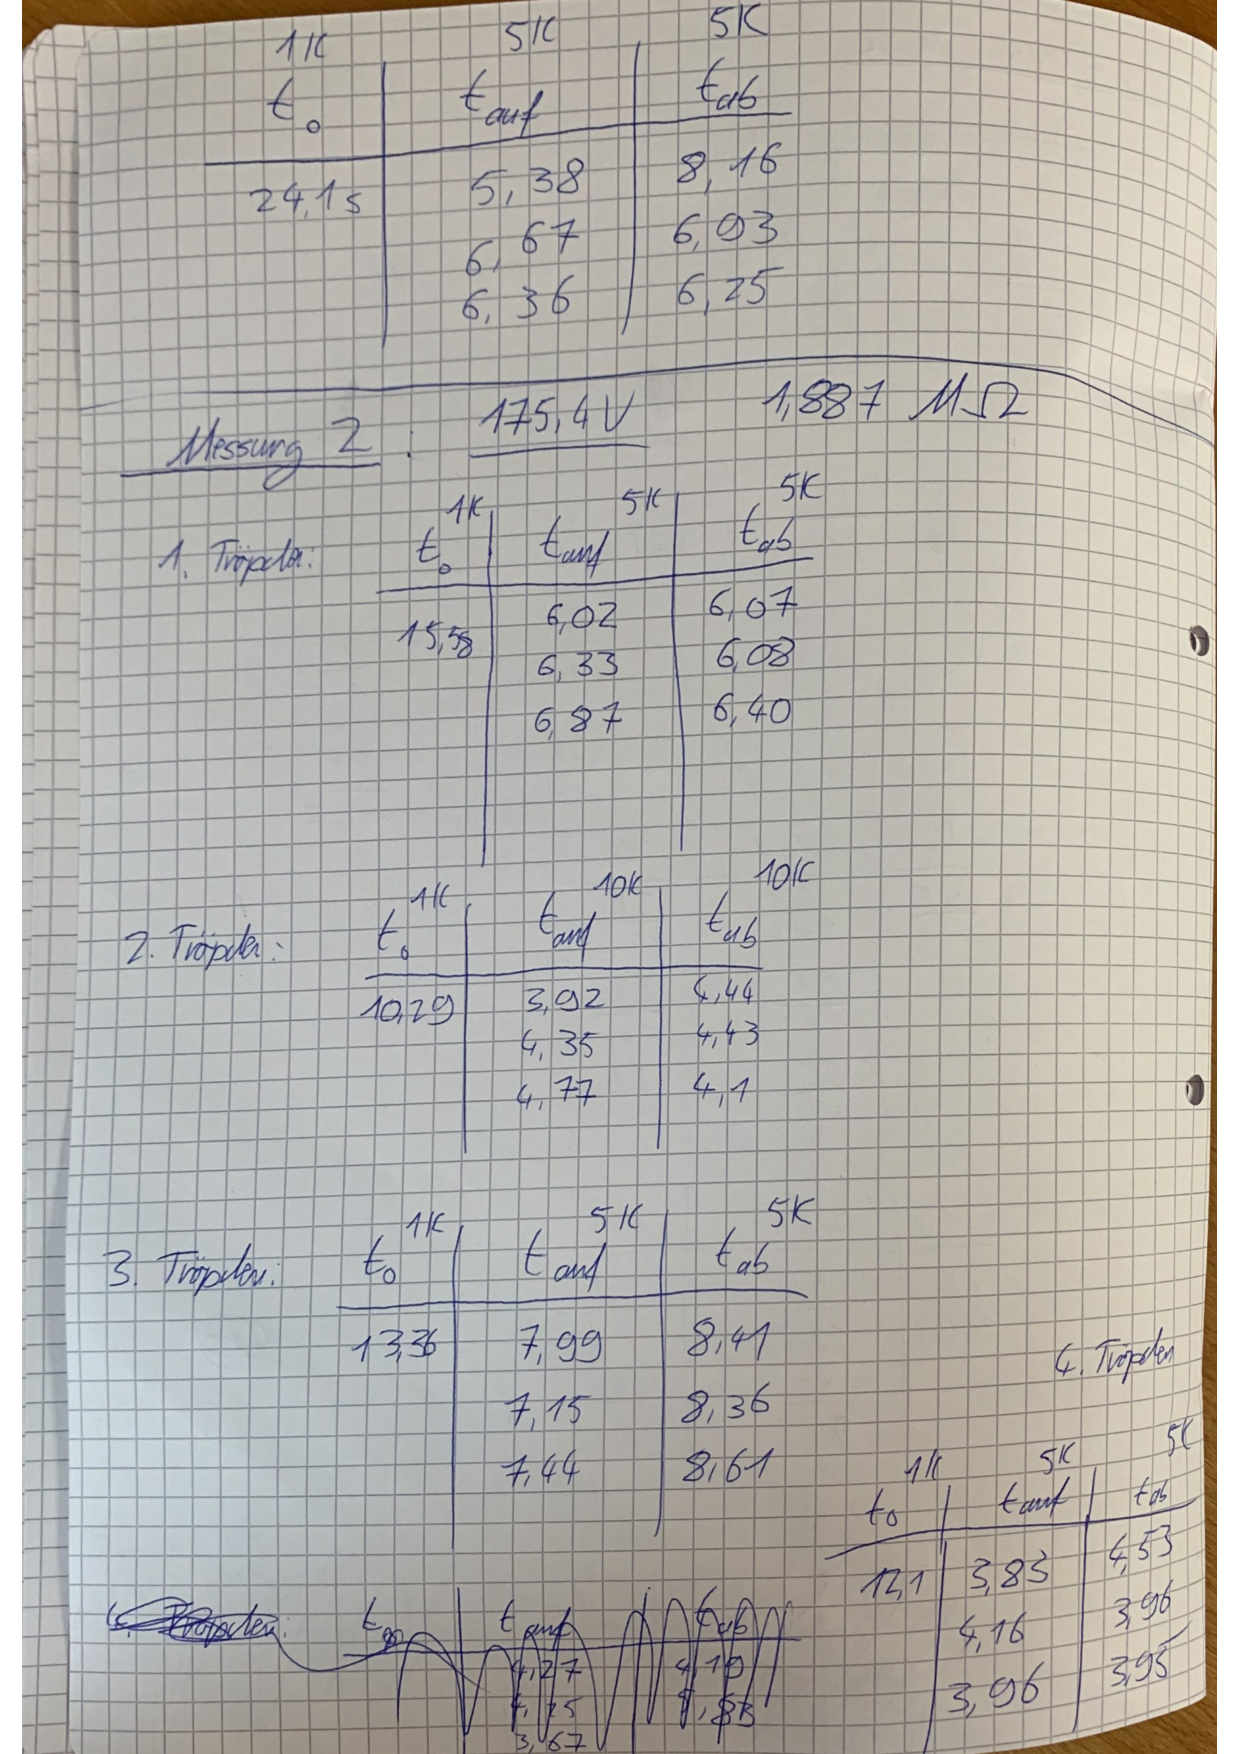
\includegraphics[height=18cm]{content/pics/originaldaten/Originaldaten_2.pdf}
\newpage
\centering
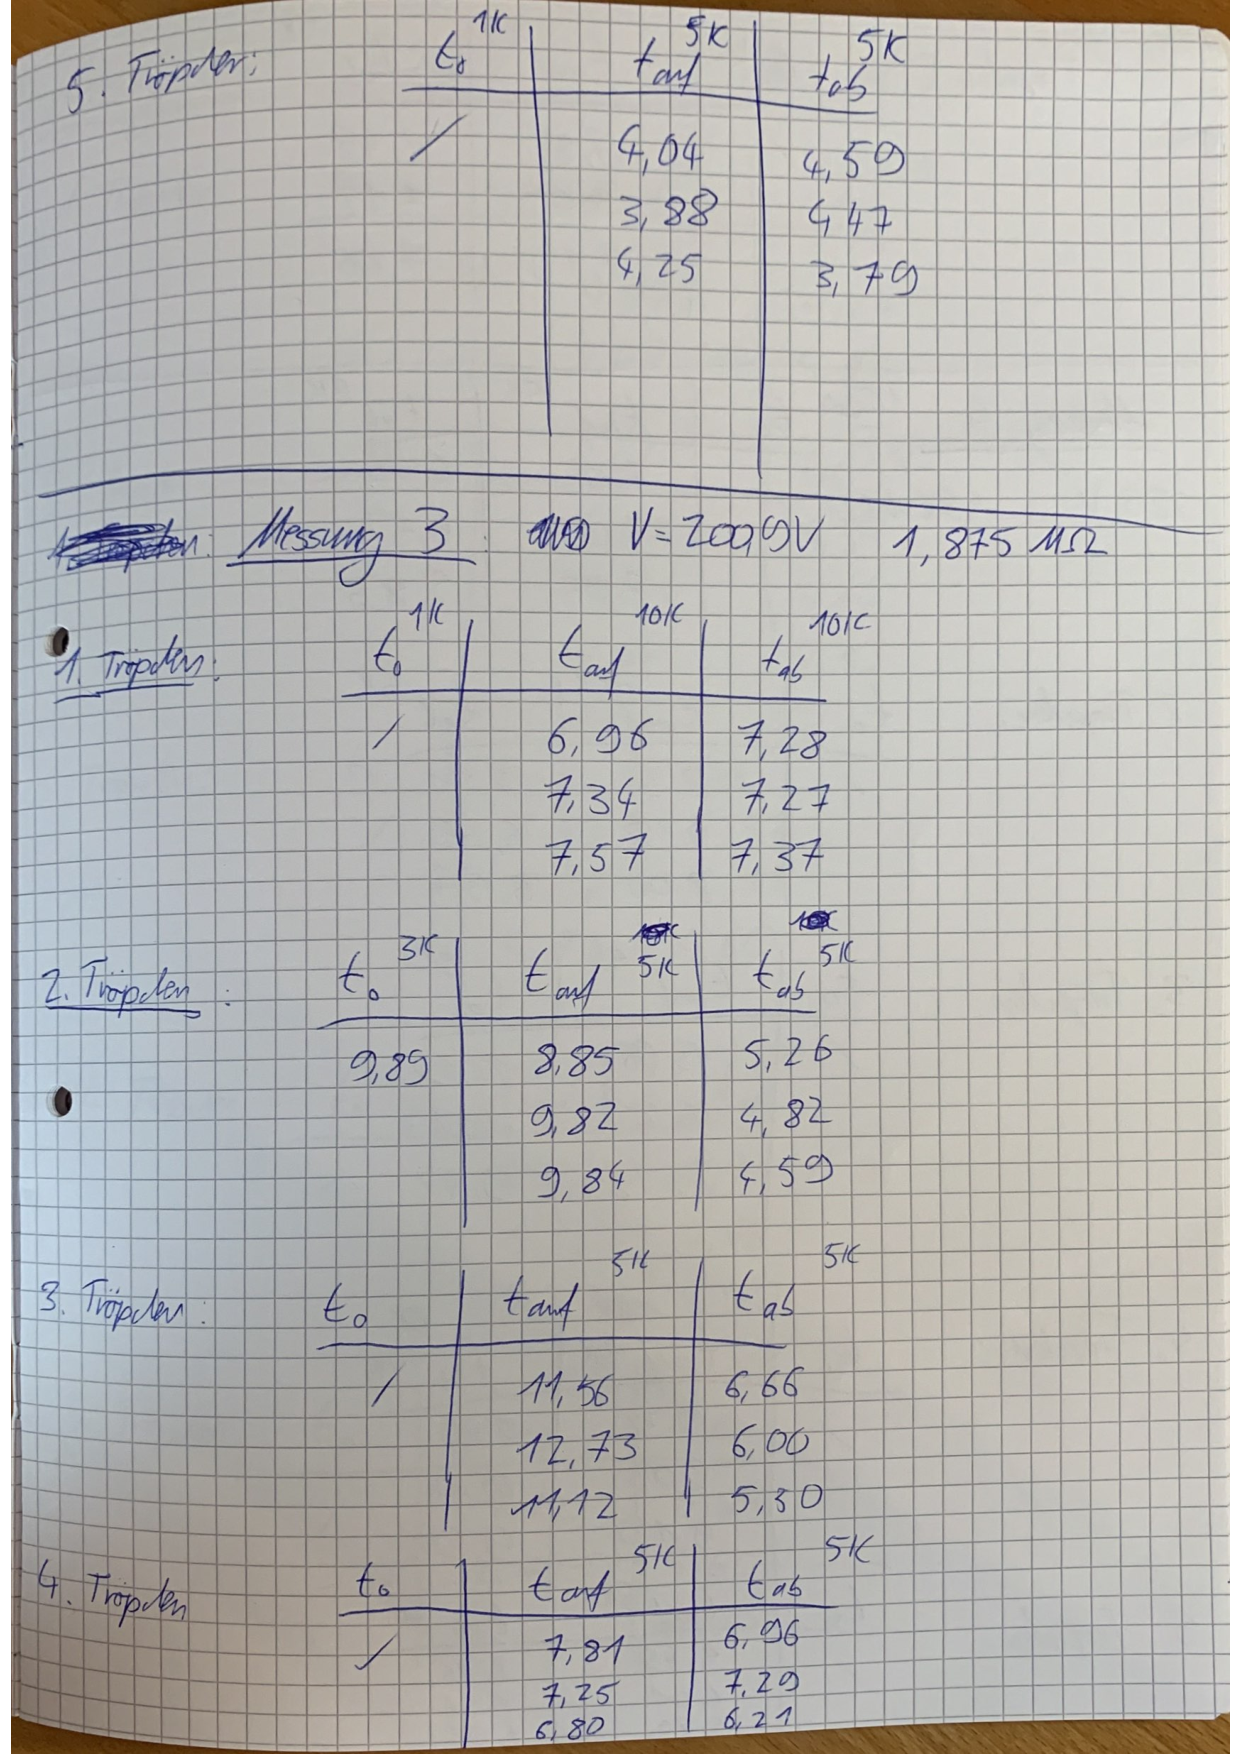
\includegraphics[height=18cm]{content/pics/originaldaten/Originaldaten_3.pdf}
\newpage
\centering
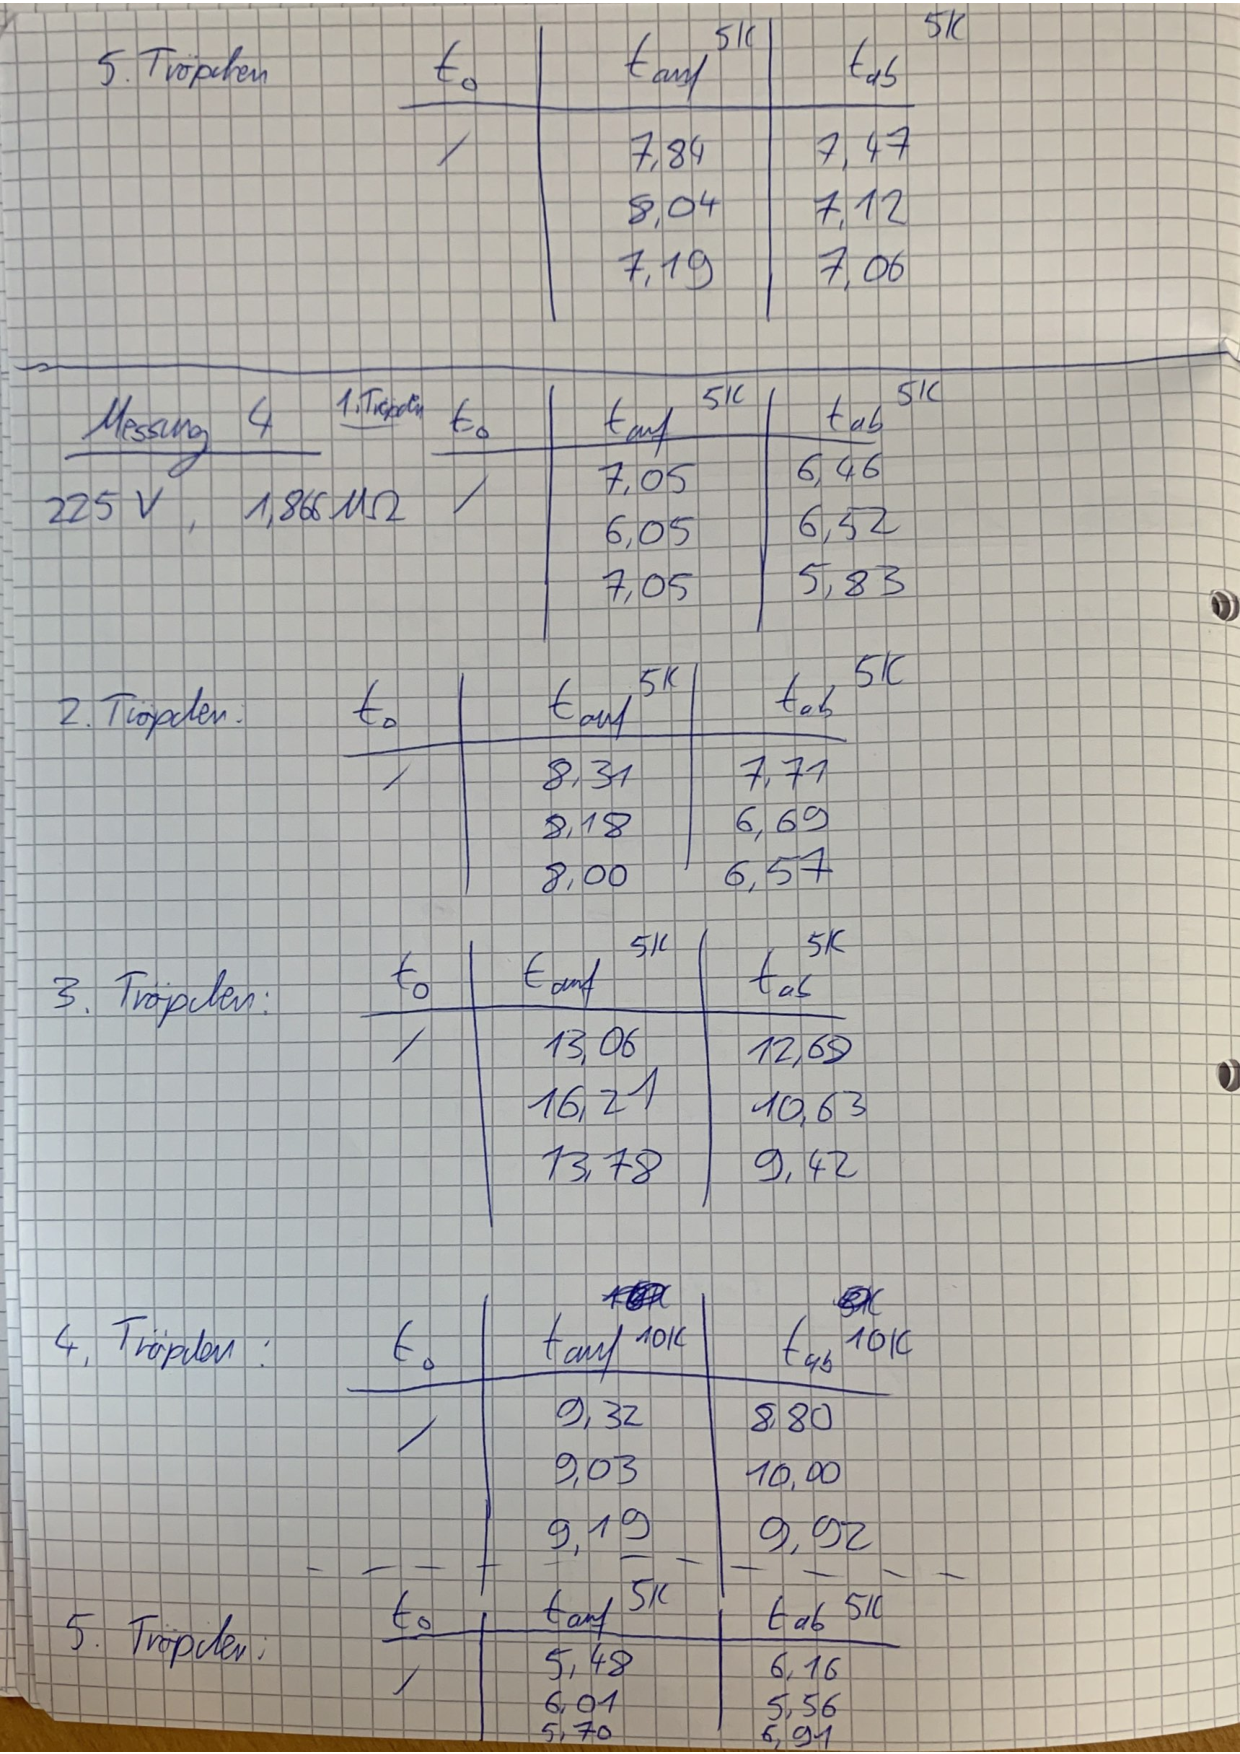
\includegraphics[height=18cm]{content/pics/originaldaten/Originaldaten_4.pdf}
\newpage
\centering
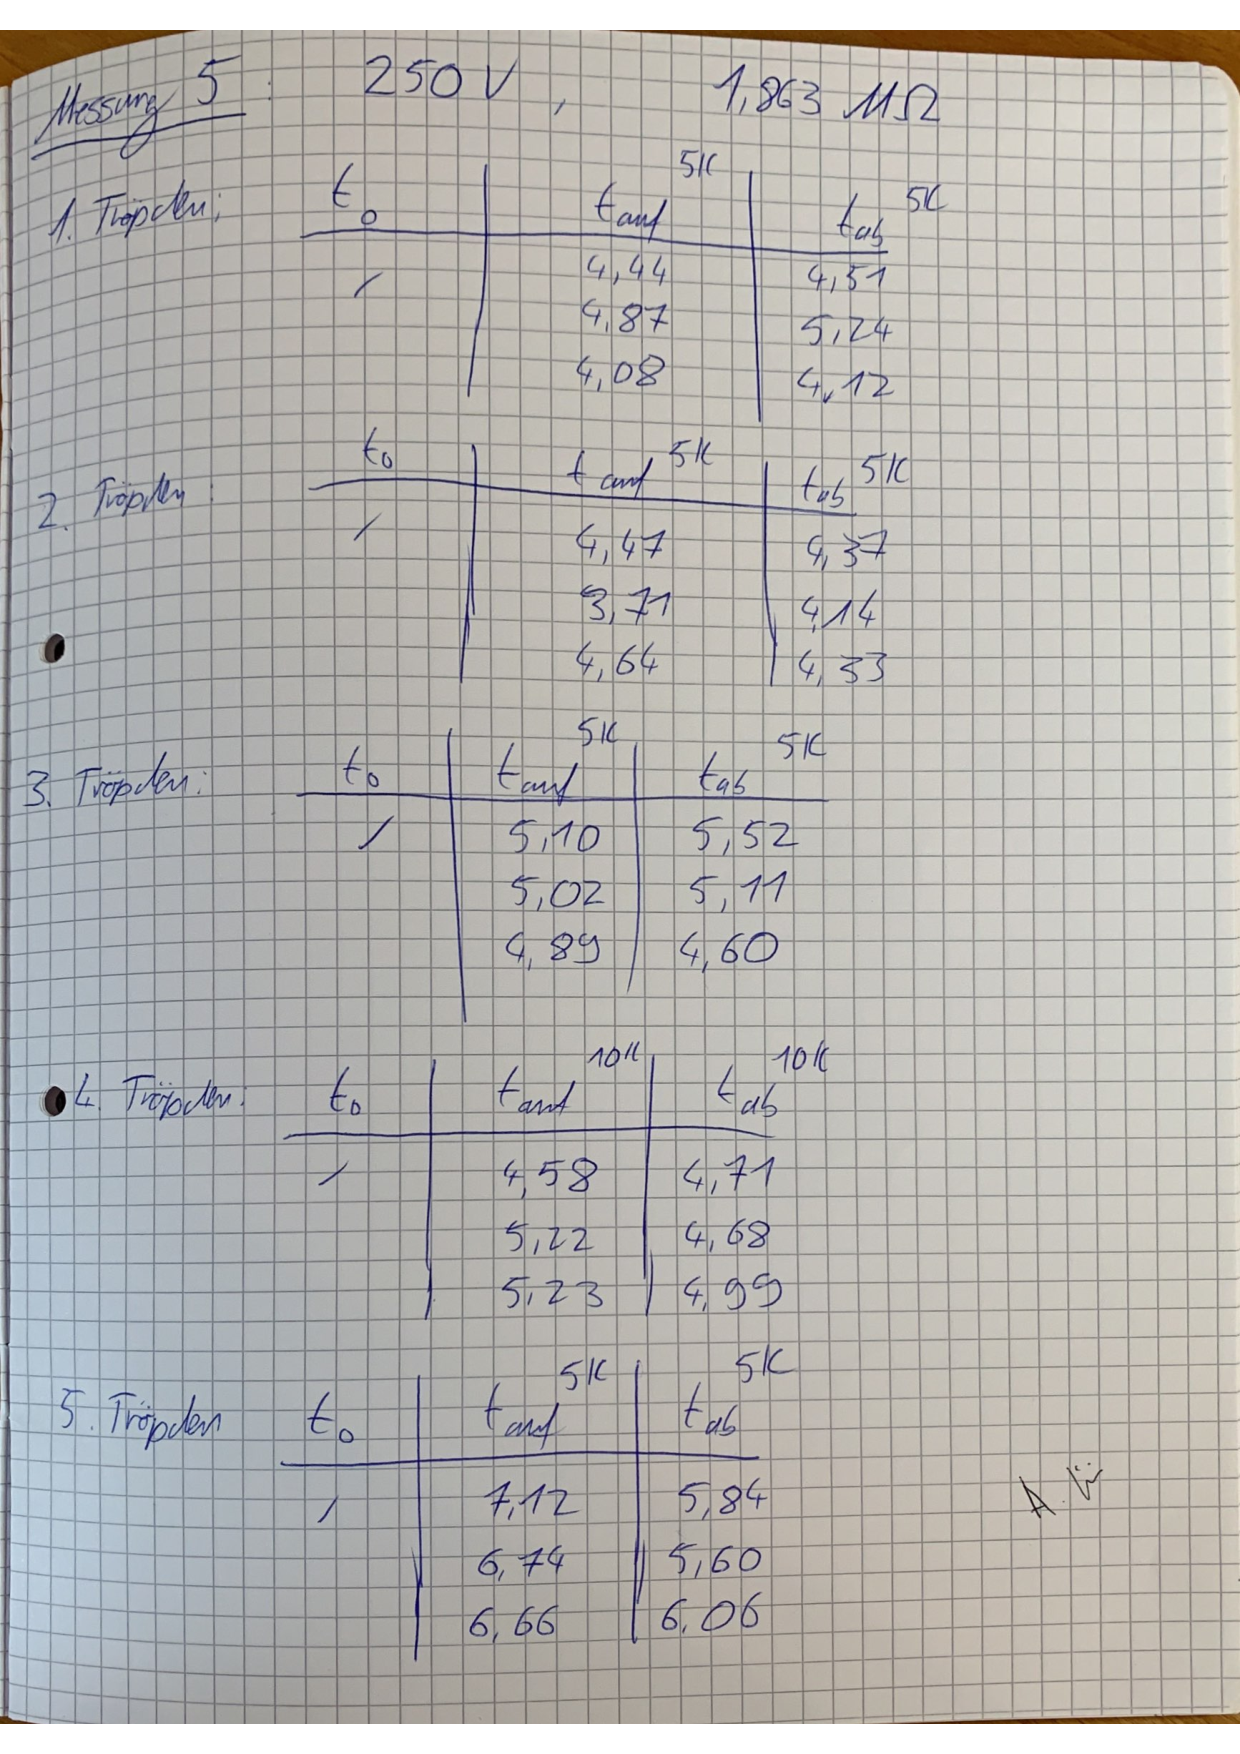
\includegraphics[height=18cm]{content/pics/originaldaten/Originaldaten_5.pdf}